\documentclass{article}
\usepackage[utf8]{inputenc}
\usepackage[margin =1.25in,includefoot]{geometry}
\usepackage{indentfirst}
\usepackage{graphicx}
\usepackage{caption}
\usepackage{tikz}
\usetikzlibrary{shapes, arrows, calc, arrows.meta, fit, trees,positioning}
\usepackage{float}

\title{COP290 Maze-Simulation}
\date{May 2021}
\author{Aniket Gupta \hspace{2cm}  Aayush Goyal \\
    2019CS10327 \hspace{2.3cm} 2019CS10452}

\begin{document}

\maketitle

\section{Minimum Spanning Tree}
\subsection{}

\begin{figure}
    \begin{center}
        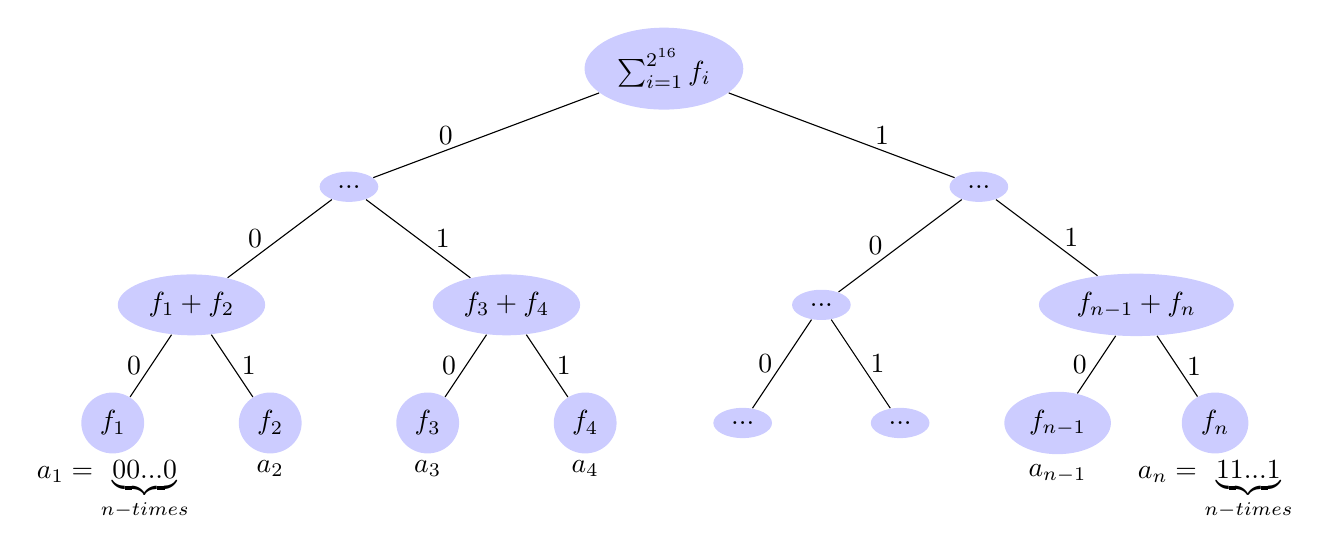
\begin{tikzpicture}[level distance=1.5cm,
            level 1/.style={sibling distance=8cm},
            level 2/.style={sibling distance=4cm},
            level 3/.style={sibling distance=2cm},
            tree node/.style={ellipse, fill = blue!20},
            every child node/.style={tree node}]
            
            \node[tree node] (Root) {$\sum_{i=1}^{2^{16}} f_i$}
                child {
                node {...} 
                child { node {$f_1+f_2$} 
                            child{ node (a1) {$f_1$} edge from parent node[left] {0}
                            }
                            child{ node (a2) {$f_2$} edge from parent node[right] {1}
                            }
                            edge from parent node[left  =0.1 cm] {0} }
                child { node {$f_3+f_4$} 
                            child{ node (a3) {$f_3$} edge from parent node[left] {0}
                            }
                            child{ node (a4) {$f_4$} edge from parent node[right] {1}
                            }
                            edge from parent node[right = 0.1 cm] {1} }
                edge from parent node[left = 0.3cm] {0} 
            }
            child {
                node {...}
                child { node  {...}  
                            child{ node (a5) {...} edge from parent node[left] {0}
                            }
                            child{ node (a6) {...} edge from parent node[right] {1}
                            }
                            edge from parent node[left = 0.1 cm] {0} }
                child { node  {$f_{n-1}+f_n$} 
                            child{ node (a7) {$f_{n-1}$} edge from parent node[left] {0}
                            }
                            child{ node (a8) {$f_n$} edge from parent node[right] {1}
                            }
                            edge from parent node[right = 0.1 cm] {1} }
                edge from parent node[right = 0.3 cm] {1}
            };
            \draw (a1) node[below = 0.35 cm,draw=none,fill=none](){$a_1=\underbrace{00...0}_{n-times}$};
            \draw (a2) node[below = 0.35 cm,draw=none,fill=none](){$a_2$};
            \draw (a3) node[below = 0.35 cm,draw=none,fill=none](){$a_3$};
            \draw (a4) node[below = 0.35 cm,draw=none,fill=none](){$a_4$};
            \draw (a7) node[below = 0.4 cm,draw=none,fill=none](){$a_{n-1}$};
            \draw (a8) node[below = 0.35 cm,draw=none,fill=none](){$a_n=\underbrace{11...1}_{n-times}$};
    
        \end{tikzpicture}
        \caption*{\textbf{Huffman encoding graph for n-bit characters}}
    
    \end{center}
    \end{figure}

\subsection{}

\section{Huffman Encoding}
\subsection{}

\subsection{}

Since these are 16 bit characters then there are a total of $2^{16}$ charcaters that are possible. We will denote $2^{16}$ by n. Let the frequencies of them be f1, f2, ... , fn, and they are in increasing order. It is given that fn $<$ 2*f1.

Now let's say we consider any numbers from them. Let them be fi and fj. 

Claim 1: fi+fj > fn (and hence greater than every other frequency). 
Proof of claim: fi >= f1
fj >= f1
and thus fi+fj >= 2*f1. 
Also it is given that fn < 2*f1, thus this directly proves that fi+ fj > fn. 

Now in huffman encoding we choose the 2 vertices with minimum frequency (say f1 and f2) and combine them. Then place a node with value f1+f2 and then recursively solve the problem further. The symbols that will be choosen in the next iteration will be f3 and f4, since f4<= f5<= fn < f1+ f2. And hence we will join f3 and f4 from the set and replace with a node of value f1+f2. This will go on and ultimately we will end with these frequencies in the set: f1+f2, f3+f4, f5+f6 ... fn-1+fn. Thus all of the symbols will be combined.

Claim 2: let f be a set of numbers of size n, here n is a power of 2. Let the numbers be f1, f2, f3, f4 .. fn-1, fn. If we make another set ff from it such that it is f1+f2, f3+f4, ... ,  fn-1+fn, then it of half the size and also follows the property that maximum element is less than twice the minimum element. 

Proof of Claim: The minimum element of ff set is f1+f2 and the maximum element is fn-1+fn. Now we know that 
fn < 2*f1
fn-1 < 2*f1
and since f1 <= f2 we can also write that fn-1 < 2*f2.
Adding both the inequalities we get fn + fn-1 < 2*(f1+ f2).

Thus for the set ff formed in the above mentioned way, the maximum is less than twice of the smallest element. 

Thus the same pattern will form here and the after combining 2 of them pairwise we will end up nodes of frequency ff1+ff2, ff3+ff4, ... , $ff_{\frac{n}{4}-1}+ff_{\frac{n}{4}}$

\section{Graduation Party of Alice}

\subsection{}
The following problem can be represented as a graph. With the n people as the nodes of the graph and there is an edge between 2 nodes if the 1 people know each other. Once the graph is ready, we can make an adjacency list for the same in O(m) time. n -> no. of people that are invited to the party and m be the no. of pairs who know each other (hence the number if edges in the graph will be m).

We can maintain an array which will store the degree if each vertex and this can be done in O(n+m) time using DFS.

Claim 1: Any node in the graph which has a degree less than 5 cannot be invited to the party. 

Now we will keep removing the nodes of the graph which have a degree of less than 5. Notice that as we remove qa vertex the degree of it's neighboring vertices will aslo change and we will update their degrees. Removing a node can cause the reduction in degree of other nodes. If the degree of those vertices fall below 5 then we can't invite them to the party either and we ill have to remove them as well. Now this process will continue untill every vertex in the graph has a degree more than 4.

Let the current number of nodes in the grpah be n'. Now consider a node whose degree is more than n'-6. Then that person doesn't know less than 5 people and we must do something in this case. 

Claim 2: Let V be the current set of nodes and n' be the size of V that is |V|. Any vertex whose degree is more than n'-6 cannot be the part of our final optimal solution. 

Proof of Claim: We will show that their is no final optimal solution in which it doesn't know atleast 5 people of all the invited people. Consider the current state of node set V. We know that the final set which will be invited to the pary is a subset of the current V. Let the node with degree more than n'-6 be v0. Now if any vertex is removed from V (which is not v0) then there are 2 possible cases. Either it is a neighbour of v0, that is it knows v0, or it is not a neighbour of v0, it doesn't know v0. If it doesn't know v0 then removing it from V only reduces the no. of people v0 doesn't know. If we remove any node which is the neighbor of v0, then removing them doesn't change the number of people v0 doesn't know. Hence the only possibility is we remove the v0.

Thus any vertex with degree more than n'-6 cannot be the part of our final solution and it must be removed from V.

Now we know that all the vertices with degree less than 5 must be removed and all the vertices with degree more than n'-6 should also be removed and this process must continue untill all the nodes left in the final V has a degree more than 4 and less than n'-6. 

Once such a V is achieved then we can show that all of these people can be invited to the party. Consider any node from the set V, let it be v1. Then v1 has a degree of more than 4 and thus it has atleast 5 neighbors and thus knows atleast 5 people who will come to the party. Also it's degree is less than n'-6 which means there are atleast 5 vertices that are not connceted to v1. Hence there are atleast 5 whom v1 doesn't know. Hence all of them can be invited to the party.

The problem can be solves in O(m log m) time using priority queue. The Pseudo code for it is wriiten below. We can initially insert all the nodes in the Priorty queue. Whenver any node is found to have a degree of less than 5 or nore than n'-6, then it is removed and marked so.  

\subsection{}

Consider all of them are standing in a sorted order of their ages. Let us call them a1, a2, a3, a4 ... , an0.  Thus we know that age[a1] <= age[a2] <= age[a3] ... <= age[an0]. Now consider the table on which a1 is sitting and let this table be T.

Claim 1: If ak is sitting on T in optimal arrangement and there exists a person (say a1) with age less than ak not sitting on T ( say they are aitting on table T1), then there also exists an optimal solution in which ak is sitting in table T1 and ai is sitting on table T.

Proof of claim: Let's say the person with age less than that of ak is ai, ak is a person sitting on the table and ai is not sitting on the table ak. Let's say ai was on the table T1. We can exchange the position of ai and ak in this case. Because: ai can be placed on table of a1 since age[ai] - age[a0] <= age[ak] - age[a0]. And we can also place ai in place of ak of ai since the leat age of a member in that is greater than or equal to age[a1] and thus the least upper bound possible is age[a1]+9 and we know that since ak was sitting on T so age[ak] <= age[a1] + 9. Thus we can always exchange ai and ak. Keeping ak in the other table can provide more flexibilty on the other table.

Now using the above we can place S  = {a1, a2, a3 ... , am} people on the first table, here m <=10 and age[am] - age[a1] <10. age[a1] <= age[a2] <= age[a3] ... <= age[am]. If m< 10 then then either we don't have enough number of people or age[m+1] - age[a1] >=10. 

Let J be the set of all the people and S be the set that we have placed. Now define J* = J \ S.

Claim 2: opt(J) = opt(J*) +1, opt(J) is the minimum number seats required to arrange the set of people J on tables under the required constraints.

Proof of Claim:
We will show that both the inequalities: 
opt(J) <= opt(J*) +1 and        ...(i)
opt(J)-1 >= opt(J*) hold.       ...(ii)

Proof of (i):
After placing S on 1 table we are left with J\S people and opt(J*) will place all of them on some table. And hence there exists one arrangement in which the arrangement can be done in opt(J*) +1 no. of tables. Thus opt(J) <= opt(J*)+1

Proof of (ii):
Let A be the optimal arrangement of J in which all the people in set S are placed on a single table and only they can be seated on that table ( say table T). Now none of the people from J\S can be seated on that table T since either T is full or their age is more than age[a1]+9. Thus the $A-T$ can be used to place all of the members of $J\S$. Thus J\S members can be placed using opt(J)-1 tables. Hence one solution of size opt(J)-1 exists for J*. This hows that opt(J*) <= opt(J)-1.

hence from both (i) and (ii) we have, opt(J)= opt(J*)+1.

Now for calculating the final we can maintain a freq array. freq[i]  denotes the number of people with age i+10. Now we can start placing them on tables in increasing order as we have discussed above, by recursively dividing the problem into a smaller sub-problem. 




\end{document}
